
% Diese ist ein Template zum Erstellen der Protokoll zum Praktikum Ein standardisierter und optimierter Prozess zur Erschließung von digitalen Herbarbelegen
% Fachgebiet Elektrotechnik und Informationstechnik, Leibniz Universität Hannover 
% 30/05/2017
% Cailin Guan 

\documentclass[10pt,a4paper]{report}

%%%%%%%%%%%%%%%%%%%%%%%%%%%%%%%%%%%%%%%%%%%%%%%%%%%%%%
%% grnutzte Package
\usepackage{ragged2e}
\usepackage{epsfig}  
\usepackage[utf8]{inputenc}
\usepackage[ngerman]{babel}
\usepackage{titlesec}
\usepackage{graphicx}
\usepackage[style=numeric-comp,backend=biber]{biblatex}
\usepackage{csquotes}
\usepackage{hyperref}
\usepackage{enumitem}
\usepackage{caption}
\usepackage{subcaption}
%%%%%%%%%%%%%%%%%%%%%%%%%%%%%%%%%%%%%%%%%%%%%%%%%%%%%%
\addbibresource{MyBib.bib}

%% ein paar kleine Modifikationen am Format
\parindent0pt                        % erste Zeile eines Absatzes nicht einrcken
\parskip 1.5ex                       % Absatzabstand
\raggedbottom                        
\renewcommand{\baselinestretch}{1.3} % Zeilenabstand

%%%%%%%%%%%%%%%%%%%%%%%%%%%%%%%%%%%%%%%%%%%%%%%%%%%%%%
%%
\titleformat{\chapter}
{\normalfont\bfseries} % format
{}{0pt}{\large}           % before-code
\titleformat{\section}
{\normalfont\bfseries} % format
{\thesection}{1em}{}        
\titleformat{\subsection}
{\normalfont\bfseries}{\thesubsection}{1em}{}
\titlespacing{\chapter}{0pt}{-50pt}{0pt}  

%%%%%%%%%%%%%%%%%%%%%%%%%%%%%%%%%%%%%%%%%%%%%%%%%%%%%%

%% Title Page
\title{Praktikumsprotokoll}
\author{Cailin Guan}
\date{\today}

%%%%%%%%%%%%%%%%%%%%%%%%%%%%%%%%%%%%%%%%%%%%%%%%%%%%%%%
%% Hier beginnt dieses Doku
\begin{document}
\maketitle  
% Erklärung für dieses Praktikum
\chapter*{Erklärung}

Hiermit erkläre ich, dass ich die vorliegende Arbeit selbst andig und ohne fremde Hilfe verfasst, und dass nur die angegebenen Quellen und Hilfsmittel verwendet wurden. Die Arbeit wurde bischer in gleicher oder änhlicher Form keineranderen Prüfungsbehörde vorgelegt.\\

Hannover, 30. Mai 2017\\

\underline{\hspace{4.5cm}}\\
Unterschrift
% Inhaltsverzeichnis	
\tableofcontents  
 
\chapter{Einleitung}

Vom September 2014 bis Mai 2017 arbeite ich in Teilzeit(33\%) an der Hochschule Hannover im Forschungsprojekt \glqq Standard Daten Akquisitionsprozess \grqq, Abkürzung \glqq stanDAP-Herb \grqq mit Visual Studio und C/C++/C\#. Dazu gehört die Entwicklung automatisierter Erkennung von Handschriftlichen Herbar - Belegen. Unter der Berücksichtigung bestehender Datenbanksystem und die Entwicklung einer funktionalen webbasierten, anwendungsorientierten Bedienoberfläche. Meinen Aufgaben zählen die digitalen Bildverarbeitung mit OpenCV Bibliothek und Programmierung, z.B GUI Oberfläche zur Web-Lokal-Steuerung, Objekterkennung mit Features, Klassifikation von multiple Objekten, Maschine Learning und Datenanalysieren wie XML und Json.\\
Ich habe am \glqq 3+1\grqq Austausch- und Kooperationsprogramm der Hochschule Hannover und der Partner Zhejiang University of Science and Technology in Hangzhou teilgenommen, und kam im Rahmen dieses Programms im Herbst 2013 nach Deutschland und belegte im WS13/14 einige englischsprachige Veranstaltung. Meine Praktikum und Bachelorarbeit absolvierte ich in diesem Forschungsprojekt \glqq stanDAP\-Herb\grqq. Danach habe ich einen Chance von Prof. Dr. Karl-Heinz Steinke bekommen, in diesem Projekt weiter zu arbeiten.\\
Das Thema \glqq Bildverarbeitung\grqq interessiert mich seit erstem Besuchen der Vorlesung \glqq Digitale Bildverarbeitung\grqq. Deshalb freute ich mich sehr, als ich die Arbeitsstelle bekam, und ich so die Möglichkeit bekam, im Rahmen dieser Teilzeitbeschäftigung arbeite ich mit zwei andere Studenten im Team zusammen. Dabei habe ich Berufserfahrung gesammelt und selbstständiges, eigenverantwortliches Arbeiten gelernt.\\

\chapter{Rahmenbedingungen}
\section{Art,Inhalt und Umfang dem Thema}

Das Projekt gehört zu Forschungsprojekt, die Grund, warum es gemacht wird, lautet, bisher werden die Metadaten von Herbarbelegen manuell in Sammlungsdatenbanken eingegeben, aber zunehmend werden Bilderfassungsverfahren eingesetzt, die auch die Nachprüfbarkeit der online verfügbaren Metainformation sichern. Das Standardverfahren soll nun so weit wie möglich die manuelle Metadatenerfassung ersetzen oder ergänzen. Bildverarbeitungssoftware erkennt Objekte auf dem digitalisierten Herbarbeleg und klassifiziert sie. Die Textobjekte werden mit Hilfe von Text - Mining Algorithmen in strukturierte Information überführt. Bei Handschriften wird versucht, den Autor zu erkennen. Im Projekt wird vorhandene Software evaluiert, unter Bildung von standardisierten Interfaces weiterentwickelt und in eine übergreifende offene Softwarearchitektur auf Grundlage etablierter IT-Standards integriert. Abschließend wird das Verfahren hinsichtlich seiner Anforderungen als Standard formuliert und hinsichtlich seiner Anwendung dokumentiert. Das Verfahren adressiert einen großen Bereich naturwissenschaftlicher Sammlungen, allein in Deutschland liegen ca. 22 Millionen Herbarbelege vor, weltweit über 500 Mio \cite{1}.\\
\begin{figure}[htbp] 
	\centering
	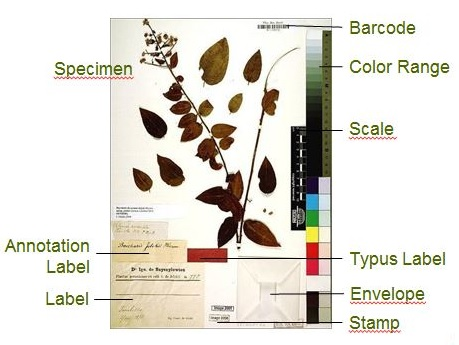
\includegraphics[width=0.7\textwidth]{Herbarbeleg_Objekte.JPG}
	\caption{Beispiel zu digitalem Bild \cite{2}, auf Herbarbelegen werden Metadaten wie Artname, Fundort und - datum, Sammler, Katalognummern etc. mit Etiketten, Barcodes usw. flächig sichtbar auf den Bogen gebracht und damit im Foto oder Scan abgebildet.}
	\label{fig:Bild1}
\end{figure}


\section{Vorstellung des Projekt: StanDAP-Herb}

Das Projekt, Standard Daten Akquisitionsprozess - Ein standardisierter und optimierter Prozess zur Erschließung von digitalen Herbarbelegen, ist durch DFG Deutsche Forschungsgemeinschaft, Literaturversorgung und Information / Erschließung und Digitalisierung gefördert, dauert insgesamt 3 Jahre lang, ab Juli 2014 bis Juni 2017. Das Ziel von diesem Projekt ist, einen softwarebasierten Standardprozess für die Extraktion von Metadaten von digitalen Herbarbelegen zu entwickeln und dokumentieren. Die Partnern von diesem Projekt sind \textit{Botanic Garden and Botanical Museum Berlin}, \textit{Fraunhofer IOSB - Karlsruhe} und \textit{Hochschule Hannover}.

\chapter{Aufgaben der Tätigkeit}
\section{Aufgabenzuteilung}

Im Rahmen des Projekt werden die Aufgaben von vier Mitarbeiten geteilt, meine Tätigkeiten im Team sind eine GUI Oberfläche zu entwickeln, um die Bilder und Metadaten zu steuern, XML Daten von OmniPage OCR Software und zu analysieren und Json Daten von gefundenen Objekten zu erzeugen. Einen kleinen Server zu bauen, um Die Lerndateien automatisch auszuschneiden. Einen SVM Klassifizierung - Server für Multiple Objekte zu bauen, und das rotes Typus zu erkennen. Für ganze Server Hunderttausend Lernbilder zu sortieren.

\section{Aufgabenbeschreibung}

Für weitere Details von meinen täglichen Aufgaben werden in der folgenden Abschnitten genauer beschrieben. 

\subsection{Microsoft Visual Studio}
Visual Studio ist eine für verschiedene Hochsprachen integrierte Entwicklungsumgebung, z.B. Visual Basic .Net, C, C++,C++/CLI, C++/CX, C\#, F\#, SQL Server, TypeScript und Python sowie HTML, JavaScript und CSS. Visual Studio ermöglicht es dem Programmierer, sowohl native Win32/Win64-Programme als auch Anwendungen für das .NET Framework zu entwickeln\cite{3}. Wir haben die Version 2008 und 2010 in Win32-Programme genutzt.
\subsection{OpenCV}
OpenCV (Open Source Computer Vision Library) ist eine freie Programmbibliothek, sie ist mit verschiedene Algorithmen für die Bildverarbeitung und Maschinelles Sehen zur Akademik und Kommerz unter eine BSD-Lizenz. Sie hat C++, C, Python und Java Oberflächen und unterstützt Windows, Linux, Mac OS, Android und IOS. Wir anwenden die Version 1.1, 2.1 und 2.4.10 für unsere Tätigkeiten.
\subsection{GUI: Web-Lokal-Steuerung}
Erste Schritte zu diesem Projekt, eine GUI Oberfläche-PLIES (Abbildung 3.1) in C\# wird entwickelt. \\ 
\begin{figure}[htbp] 
	\centering
	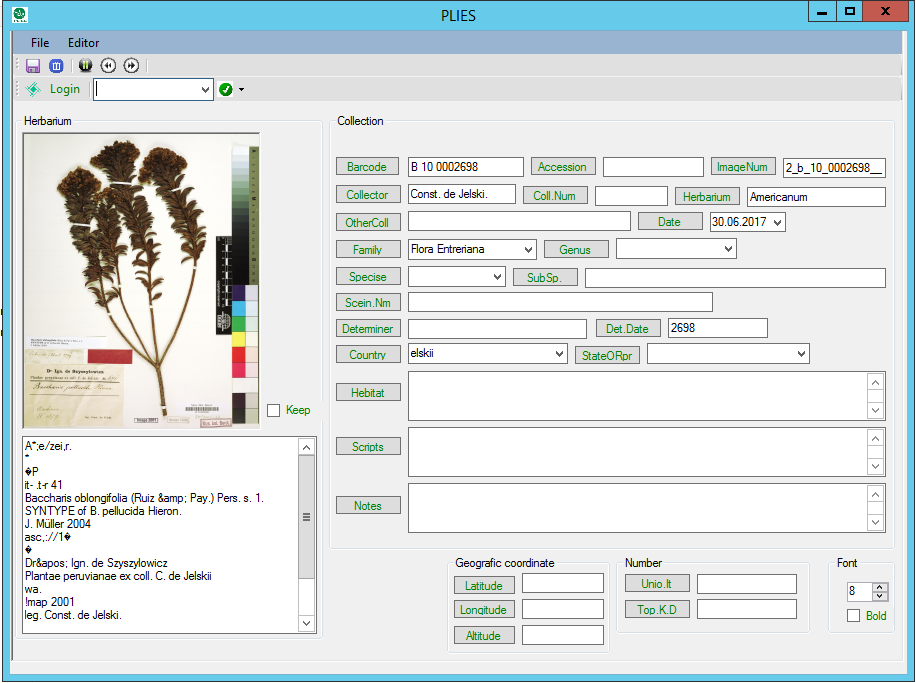
\includegraphics[width=0.6\textwidth]{GUI.png}
	\caption{GUI-Oberfläche}
	\label{fig:Bild 3.1}
\end{figure}\\
Mit Hilfe dieser Oberfläche können die Bild und von OCR-OmniPage Software extrahierter TXT/XML Datei automatisch von OCR-Server hochgeladen werden.
und XML Parsing, Fuzzy Search und mit Rest Service verbunden sein. Mit eine Funktion \glqq Log in\grqq kann auch mit dem Server von \textit{Fraunhofer IOSB - Karlsruhe} \href{https://standap-herb.server.de/servlet/is/11/}{https://standap-herb.server.de/servlet/is/11/} verbunden sein, um die Bilder von \textit{Botanic Garden and Botanical Museum Berlin} automatisch herunterladen und das Ergebnis von \textit{Hochschule Hannover} hochladen. Damit können auch z.B. die Metainformationen mit Regex(regulärer Ausdruck, englisch regular expression),das ist in der theoretischen Informatik eine Zeichenkette, die der Beschreibung von Mengen von Zeichenketten mit Hilfe bestimmter syntaktischer Regeln dient, wegen ihren Einträge oder Abkürzungen weiter bearbeitet werden,Abbildung 3.2,dadurch können der fehlerbehaftet OCR-Server sich ausgleichen.\\
 \begin{figure}[htbp] 
 	\centering
 	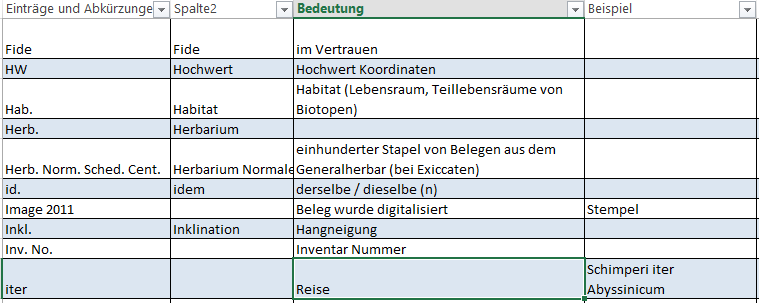
\includegraphics[width=0.7\textwidth]{Regex.png}
 	\caption{Einträge oder Abkürzungen}
 	\label{fig:Bild 3.2}
 \end{figure}\\
Bevor der Verwendung von Regex muss die extrahierte XML Datei aufgrund ihre hohe Sicherheit und Standardisierung vergleichen zur TXT Datei zuerst analysiert werden, sogenannt XML Parsing. 

\subsection{Fuzzy Search}
In der Computer Wissenschaft gibt es eine Suche Methode, nennt man unscharf Suche bzw. Fuzzy-Suche, ist eine Technik von Suchen eine bestimmte Zeichenkette in einer längeren Zeichenkette oder einem Text. Es geht sich um Matching Algorithmen, ein bekanntes Algorithmus zur Berechnung ist die sogenannt Levenshtein-Distanz, die auch in der Oberfläche PLIES verwendet werden.  
Durch die Fuzzy-Suche können die von Regex bearbeitete Metainformationen  automatisch die entsprechende richtige Information von außen verbunden Server genau gefunden und weiter mit diese Oberfläche als XML Datei gespeichert werden. Beispielsweise Server: GeoNames geographical database (\href{http://geonames.org/}{http://geonames.org/}), JRZ fuzzy gazetteer (\href{http://dma.jrc.it/services/fuzzyg}{http://dma.jrc.it/services/fuzzyg}), Sammlernamen (\href{http://kiki.huh.harvard.edu/databases/botanist\_index.html}{http://kiki.huh.harvard.edu/databases/botanist\_index.html}).

\subsection{Rest Server}
Representational State Transfer web Service, abgekürzt Rest oder ReST, ist eine Möglichkeit der Interoperabilität zwischen Computersystemen im Internet. Das Ziel ist, einen Architekturstil zu schaffen, der die Anforderungen des modernen Web besser darstellt.
Um die Teilen von diesem Projekt schnell und nahtlos zu kommunizieren und konfigurieren, bei uns viele Rest Server gebaut werden. z.B. Land-Suche Dienst Server, Tamplate Matching Dienst Server, Furzzy Search Dienst Server usw..
es gibt zwei neuen Endpoints im StanDAP-Herb Server, hier ist Paar Beispiel dafür, Server : \href{http://hsh.iosb.fraunhfer.de/}{http://hsh.iosb.fraunhfer.de/}
\begin{itemize}
 \item POST /api/herbariums/country/txt
 \item POST /api/herbariums/country/xml
\end{itemize}
Suchen nach Länder mit der hochgeladenen XML/TXT Datei. Damit der Dienst den Inhalt der XML-Datei richtig interpretieren kann, kann es notwendig sein, die Codierung anzugeben. Zum Beispiel mit "text / xml; charset = utf-16" in Inhaltstyp.Standardmäßig werden die Ergebnisse in XML zurückgegeben. Setzen Sie auf "application / json", um die Ergebnisse im JSON-Format zu erhalten.
\begin{itemize}
\item POST /api/herbariums/images/typus?ID={imageId}\&Type={type}\\
\begin{figure}[htbp] 
	\centering
	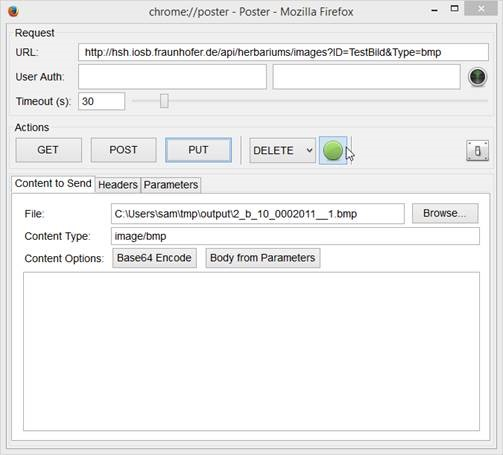
\includegraphics[width=0.5\textwidth]{RestServe1.jpg}
	\caption{RestServe-Post: Suchen nach Typus im Bild. Rückkehr Token für späteren Download der Ergebnisse}
	\label{fig:Bild 3.3}
\end{figure}
\item GET /api/herbariums/images/typus/matches/files?ID={imageId}\&Type={type}\&Token={token}
\begin{figure}[htbp] 
	\centering
	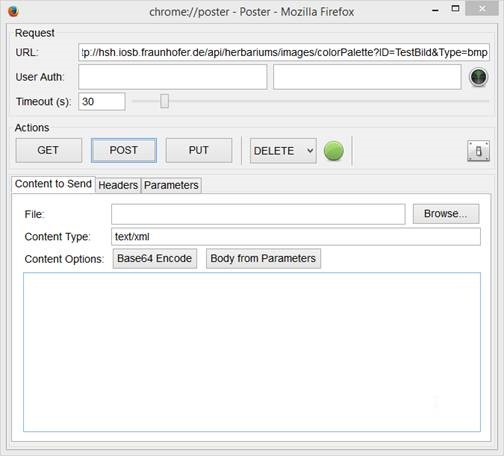
\includegraphics[width=0.5\textwidth]{Server2.jpg}
	\caption{RestServe-Get :
	Holen Sie sich die Ergebnisse der Typus-Extraktion. Needs token zur Verfügung gestellt von vorherigen Post Anfrage..}
	\label{fig:Bild 3.4}
\end{figure}
\item Result \\
\begin{figure}[htbp] 
	\centering
	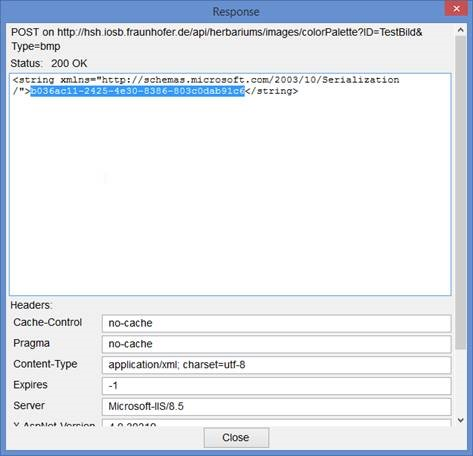
\includegraphics[width=0.4\textwidth]{Server3.jpg}
	\caption{RestServe-Result: Zeigen das Resultat von Dienst Server}
	\label{fig:Bild 3.5}
\end{figure}
\end{itemize}
Im Hintergrund läuft das entwickelte DLL. Die DLLs kann sehr nützlich sein, um die Entwicklung von anderen Diensten zu unterstützen.

\subsection{Auto-Cut}
Es gibt viele Objekte auf eine Herb-beleg, z.B. Barcode, Stampe, Typus…, die wir erkennen sollen. Eine Seite kann das ganze Bild in Server (OCR) laufen, um Informationen zu extrahieren, andere Seite, es ist auch wichtig, die einzeln Objekt in Server behandeln, damit kann die Anerkennungsquote zu erhöhen. Deswegen brauchen wir riesige Menge Ausschneiden von den Objekten.
Um das Aus schneiden durchzuführen, müssen wir überlegen, wie es machen kann. Natürlich können wir das Ausschneiden manuell durch Paint oder GIMP erledigen, aber es ist offensichtlich, zeitaufwändig. Anstatt die Objekte aus Herb-Beleg selbst per Hand auszuschneiden, ist es nötig, ein kleines Programm zu entwickeln, damit kann man sehr effizient im kurzen Zeitraum viel Objekte erhalten. 
Bild ist durch das Programm hochgeladen worden, und durch Maus das Objekt abzugrenzen, z.B. bei einem Barcode klicken wir mit der linken Maustaste auf den oben links Punkt und ziehen wir bei gedrückter Maustaste bis zum unten rechts Punkt, danach lassen wir die Maustaste los. Damit bekommen wir die Koordinaten von den beiden Punkten, schneiden die Rechtangle, die die Punkte bezüglich ist, aus.\\
\begin{figure}[htbp] 
	\centering
	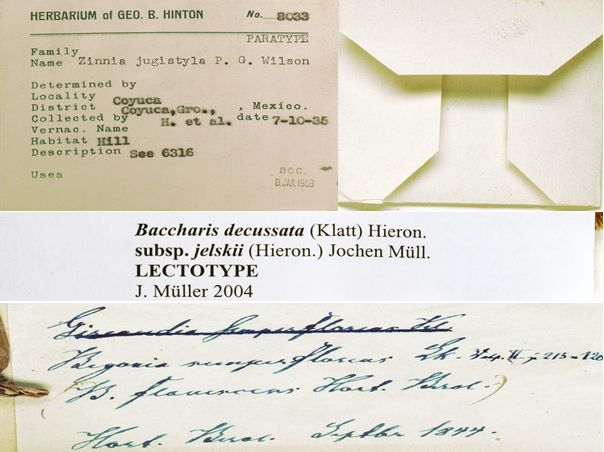
\includegraphics[width=0.4\textwidth]{Cutobjekte.png}
	\caption{Objekte Belege}
	\label{fig:Bild 3.6}
\end{figure}\\
Speichern sollen wir auch berücksichtigen, um die Objekte später direkt zum Anlernen genutzt zu werden. Brauchen wir Sortierung während Speichern, z.B. bei dem Objekt Barcode, drucken wir die Tastatur „3“, damit das Barcode würde automatisch im dritten Datei gespeichert werden. Die ausführlichen Informationen von „Objekt-Tastatur-Speicherdatei“  sind in folgende Tabelle gegeben, sehen Sie Abbildung 3.7.\\
\begin{figure}[htbp] 
	\centering
	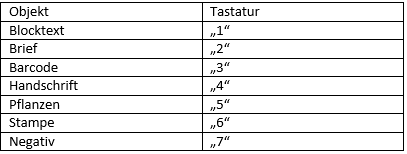
\includegraphics[width=0.5\textwidth]{Tabelle.png}
	\caption{Objekt-Tastatur-Speicherdatei}
	\label{fig:Bild 3.7}
\end{figure}\\
Der Tabelle zeigt genau bei welchem Objekt sollen wir welche Tastatur drucken, um das Objekt richtig zu speichern.

\subsection{HSV-Farbraume}
Der HSV-Farbraum ist ein Farbraum etlicher Farbmodelle, bei denen man kann die Farbe mit Hilfe des Farbwerts (englisch hue), der Farbsättigung (saturation) und des Hellwerts (oder der Dunkelstufe) (value) definieren(Abbildung 3.8) \cite{7}. \\ 
\begin{figure}[htbp] 
	\centering
	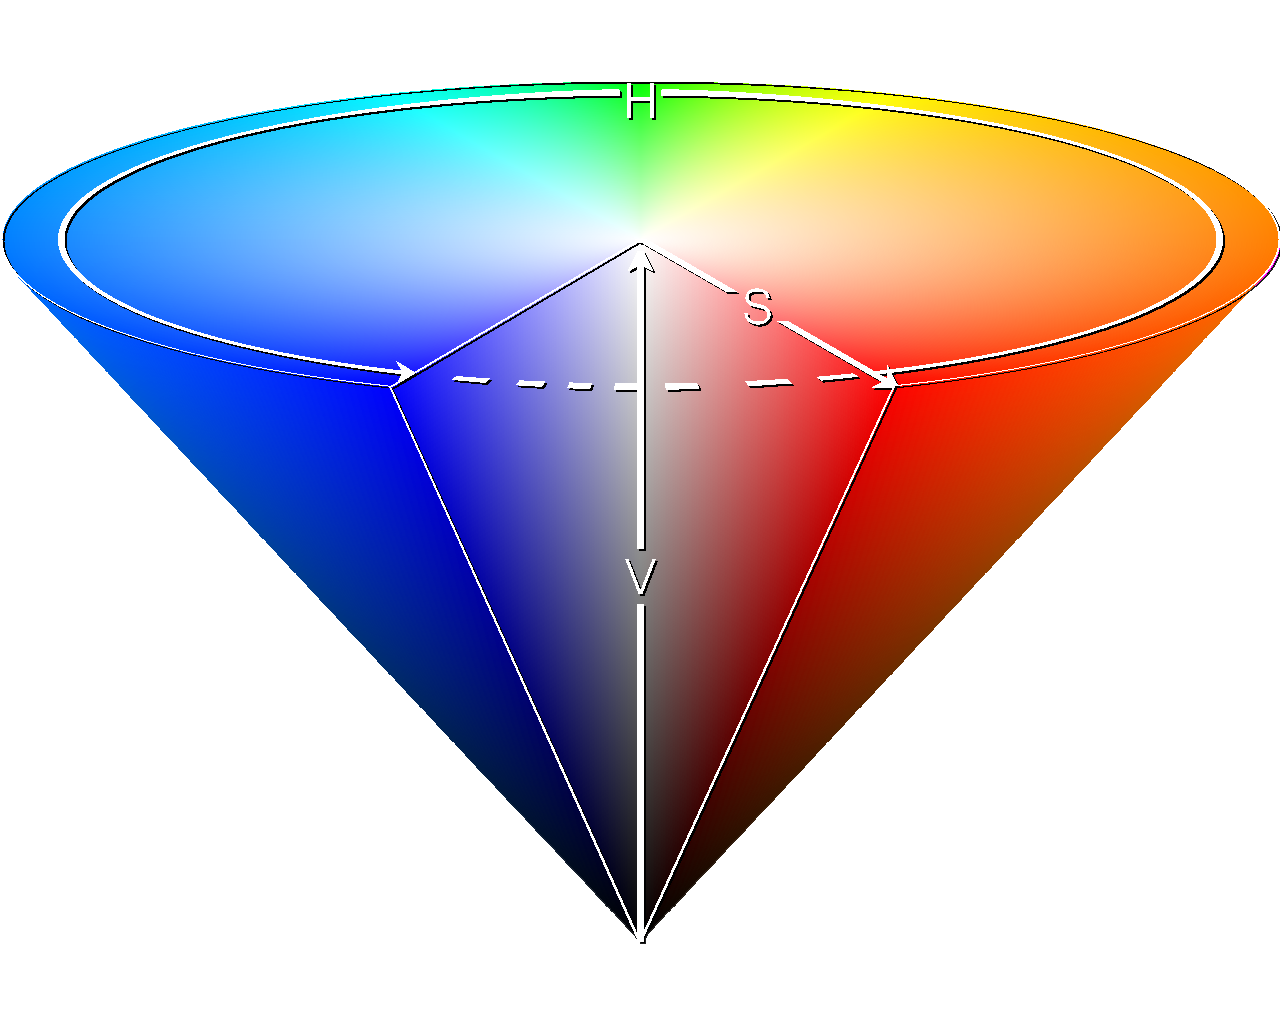
\includegraphics[width=0.3\textwidth]{HSV_cone.png}
	\caption{HSV-Farbraum als Kegel}
	\label{fig:Bild 3.8}
\end{figure}\\
Mit diese Objekte von Typus habe ich diese Farbraum Modell wegen ihrer speziellen Farbe, normalerweise sind die immer rot(Abbildung 3.9), angewendet. Damit nur die Farbekanal von Rot ausgefiltert werden.\\
\begin{figure}[htbp] 
	\centering
	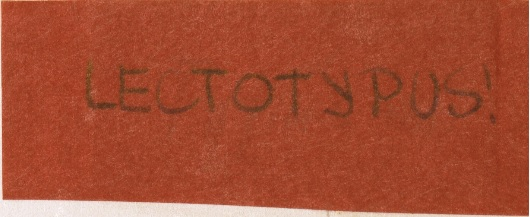
\includegraphics[width=0.4\textwidth]{test.jpg}
	\caption{Beispiel von Typus}
	\label{fig:Bild 3.9}
\end{figure}


\subsection{Segmentierung}
Ermittlung von Rechtangle ist der Prozess, ein Bild in multiple Segmentation zu trennen. Dieser Prozess dient dafür, Analysierung von Bild und Extraktion von Merkmal zu vereinfachen.\cite{5} 
In unsere Situation ist das wichtige Merkmal von Segmentation vertikal Kante in dem Bild, der Merkmal kann ausgenutzt werden und die Regionen, die gar keine vertikale Kante haben, zu eliminieren. 
Bevor Finden der vertikale Kante, sollen wir die mögliche Rausch mit Gaussian blur möglich viele entfernen. Um die vertikale Kante zu finden, haben wir uns die Sobel Filter entschieden. Weil mit diese Funktion können wir selbst Richtungsderivat definieren. 
Nach Sobel Filter bieten wir eine Threshold Funktion, um das Bild zum Binary zu transformieren. Und danach durch Morphologische Operation können wir den Spalt zwischen Kante eliminieren und die andere nötige Kante verbinden. In unsere Situation liefert es bei der Dimension 41x30 ein gutes Ergebnis. Aber wir lassen das veränderbar, weil für uns die Bilder immer Variante ist, mit verschieden Leuchtdichte, verschiedenen Lokalisation der Objekten, manchmal sehr eng miteinander, manchmal gibt es genug Abstand zueinander, und natürlich mit verschiedenen Klarheit von den Objekten, deswegen hat die Dimension von morphologischer Operation sehr groß Beeinflusse, zu groß oder zu klein würden die Objektregionen nicht mehr finden können. Beispielweise die Abbildung 3.10).\\
\begin{figure}[htbp] 
	\centering
	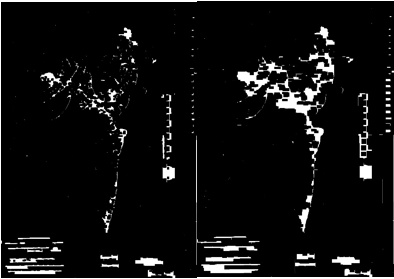
\includegraphics[width=0.5\textwidth]{SVMPre.png}
	\caption{Verschneiende Bilder zu vergleichen}
	\label{fig:Bild 3.10}
\end{figure}\\
Links Bild mit Dimension 41x30 ist für Stampe besser, aber recht Bild ist mit Dimension 80x45 ist für Mus.Bot.Berol besser. Man kann nicht nur mit einer bestimmten Dimension alles gewonnen.
Konturen sollen dann mit dem resultierenden Bild gefunden werden. Damit erhalten wir aber viele Müll, deswegen sollen wir die Segmentation überprüfen. Mit definiertem Seitenverhältnis, In unsere Situation ist es 3.8 mit 40\% Fehlertoleranz, können wir Stampe, Barcode, Mus.Bot.Berol alle ausfinden. Die Richtung der Segmentation ist auch berüchtigt, d.h. die in beide Richtungen liegende Segmentation können herausgefunden werden.
Für Typus ist nichts anderes als Stampe, Barcode, außerdem von Beginnen werden die HSV genutzt, weil der Typus ist alles rot oder ähnlich rot. Danach mit 5x5 Dimensionen morphologische Operation, und Seitverhältnis 2.5 mit 40 Fehlertoleranz.
Die alle gefundenen möglichen Objektregionen würden auch sortiert, und parallel muss gespeichert werden. Z.B. Tastatur „0“ bezüglich auf nicht interessierte Objektregion, Tastatur „1“  bezüglich auf Stampe, Tastatur „2“ bezüglich auf Mus.Bot.Berol, und Tastatur „3“ bezüglich auf Barcode.  


\subsection{SVM-Klassifikator}
SVM ist eine Support Vector Machine, die als Klassifikator(vgl. Klassifizierung) und Regressor (vgl. Regressionsanalyse) dient. Eine SVM unterteilt eine Menge von Objekten so in Klassen, dass um die Klassengrenzen herum ein möglichst breiter Bereich frei von Objekten bleibt, sie ist ein sogenannter Large Margin Classifier (engl. „Breiter-Rand-Klassifikator“). SVMs können sowohl zur Regression als auch zur Klassifizierung verwendet werden\cite{4}.
SVMs sind keine herkömmliche Maschinen zu verstehen. Die bestehen  nicht aus greifbaren Bauteilen, sondern handeln sie sich um ein rein mathematisches Verfahren der Mustererkennung, das in Computerprogrammen umgesetzt wird. Der Namensteil Machine weist dementsprechend das Herkunftsgebiet der Support Vector Machines, das maschinelle Lernen.
In unsere Programm verwenden wir SVMs nur zur Klassifizierung, die darstellte Abbildung 3.11 zeigt, wie sollen wir die Objekte erkennen. In dem SVM Programm definieren wir drei wichtige Funktionsschritte, unser System zu trainieren.\\
\begin{figure}[htbp] 
	\centering
	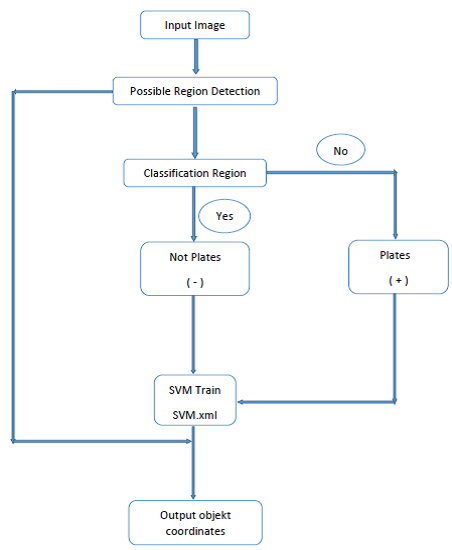
\includegraphics[width=0.5\textwidth]{SVM.png}
	\caption{SVM Programm : Dieses ganze Prozesses beziehen sich auf das Programm sind Sobel Filter, Threshold Operation, Morphologic Operation, Find Contours, SVM Klassifikation, SVM Training.}
	\label{fig:Bild 3.11}
\end{figure}\\
Die alle gespeicherten Objektregionen, sollen wir entscheiden, dass ob die gefundene Objektregion eine Stampe oder ein Barcode ist. Um dies zu erledigen, brauchen wir jetzt SVM Algorithmus. 
Bevor der Klassifikation muss der Klassifikator mit Label trainiert werden, sog. Offline Training. In unsere Situation, wegen der vielen varianten Bilder brauchen wir eine ausreichende Menge Daten zu trainieren. D.h. je größer unsere Datenbank ist, umso kriegen wir besser Ergebnis. Deswegen brauchen wir zu mindesten ein paar tausend Herb-Beleg für Preprozessor und Segmentierung.
SVM ist inhärent ein binärer Klassifikator, in unsere Situation, für Stampe, Barcode, Mus. Bot. Berol. bedürfen wir 4 Klasse, wir nutzten lineare Klassifikation. Es gibt viele Möglichkeiten zu trainieren, z.B. one-versus-rest(OVR SVMs), one-versus-one (OVO SVMs). Wir haben uns OVR SVMs entschieden, weil für uns ist es sehr schnell und unser System ist nicht kompliziert. Unser Prozess beruht sich auf die Bildpixels, sehen Sie in folgendem Bild(Abbildung 3.12).\\
\begin{figure}[htbp] 
	\centering
	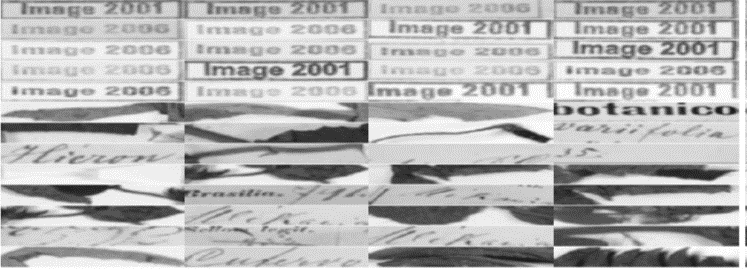
\includegraphics[width=0.7\textwidth]{Positivnegativ.png}
	\caption{Positive Bilder und negative Bilder}
	\label{fig:Bild 3.12}
\end{figure}\\
Klasse Stampen gegen die andere, Stampe werden als positivem Label identifiziert, die andere werden als negativem Label identifiziert. Barcode, Mus.Bot.Berol werden auch so trainiert. Dann die ganzen trainierten Daten  werden in eine XML Datei gespeichert.

Nach dem Bekommen der trainierten Daten müssen wir jetzt die SVM Parametern definieren, um das SVM Algorithmus zu verwenden. In OpenCv ist es einfach, dass wir können einfach CvSVMParam direkt anrufen und die Parameter eingeben. Hier könnten wir auch die Parameter automatisch mal trainieren, um die besten Parametern zu erzielen\cite{6}. 
Mit eingegebenen Parameters kann die Klassifikator trainieret werden. Danach ist es bereit zu Prognose von möglichen Objektregionen mit Predict Funktion. Falls wir positive Resultat erhalten, ist die Objektregion interessiert uns, negative Resultat, dann interessiert uns nicht. Somit können wir klassieren alle gefundenen möglichen Objektregionen mit der Rückmeldung von Prognose. Nur die mit dem positiven Prognose Objektregionen und auch deren Koordinaten werden gespeichert(Abbildung 3.13). \\
\begin{figure}[htbp] 
	\centering
	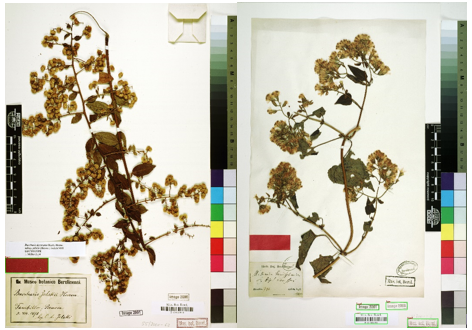
\includegraphics[width=0.5\textwidth]{Svmresult.png}
	\caption{Resultat von SVM Programm: Die Abbildung zeigt, wie das Resultat von SVM Programm im originalen Bild aussieht, die mit grünen Rechtangle eingehüllten Objekte sind die gefundenen Objekteregionen. Links ist für Typus, rechts ist für Stampe, Barcode, Mus.Bot.Berol.. Die gespeicherten Koordinaten werden weiter in andere Programm geliefert.
	}
	\label{fig:Bild 3.13}
\end{figure}

\subsection{Automatischer Objekterkennung}
Um die Koordinaten auf Herb-Beleg zu erhalten, automatische Erkennung von den Objekten ist in der erste Linien.  Dieses Programm ist genau dafür gesorgt. Es beinhaltet Ermittlung von Objekt(Preprozessor), und Klassifikation von Objekte.  Das Ziel von Ermittlung dem Objekt ist es, die möglichen Objektregionen in ganzen Bildframe zu ermitteln. Falls eine Rechtangle wird ermittelt, die Rechtangle Segment wird in den zweite Schritt übertragt, mit SVM(Support Vector Machine) Algorithmus zu entscheiden, ob die Rechtangle richtig ist. Durch das Programm können die Koordinaten von Objekt automatisch geliefert werden. Die Koordinaten können später in andere Programm eingeben, um die Region automatisch zu ausschneiden. 

\subsection{Json}
Json, JavaScript Object Notation ist ein leichtes Datenaustauschformat, es ist einfach für Menschen zu lesen, schreiben, analysieren und generieren. Es basiert auf einer Teilmenge der JavaScript-Programmiersprache, Standard ECMA-262 3. Auflage - Dezember 1999\cite{8}. JSON ist ein Textformat, das vollständig sprachunabhängig ist, aber verwendet Konventionen, die den Programmierern der C-Familie von Sprachen vertraut sind, einschließlich C , C ++, C\#, Java, JavaScript, Perl, Python und viele andere. Diese Eigenschaften machen JSON zu einer idealen Datenaustauschsprache.\\
Nach Automatischer Objekterkennung sollen die Koordinaten von erkannten Objekte gespeichert werden(Abbildung 3.14), um diese entsprechende Objekte in andere Dienst Server automatischer auszuschneiden. \\
\begin{figure}[htbp] 
	\centering
	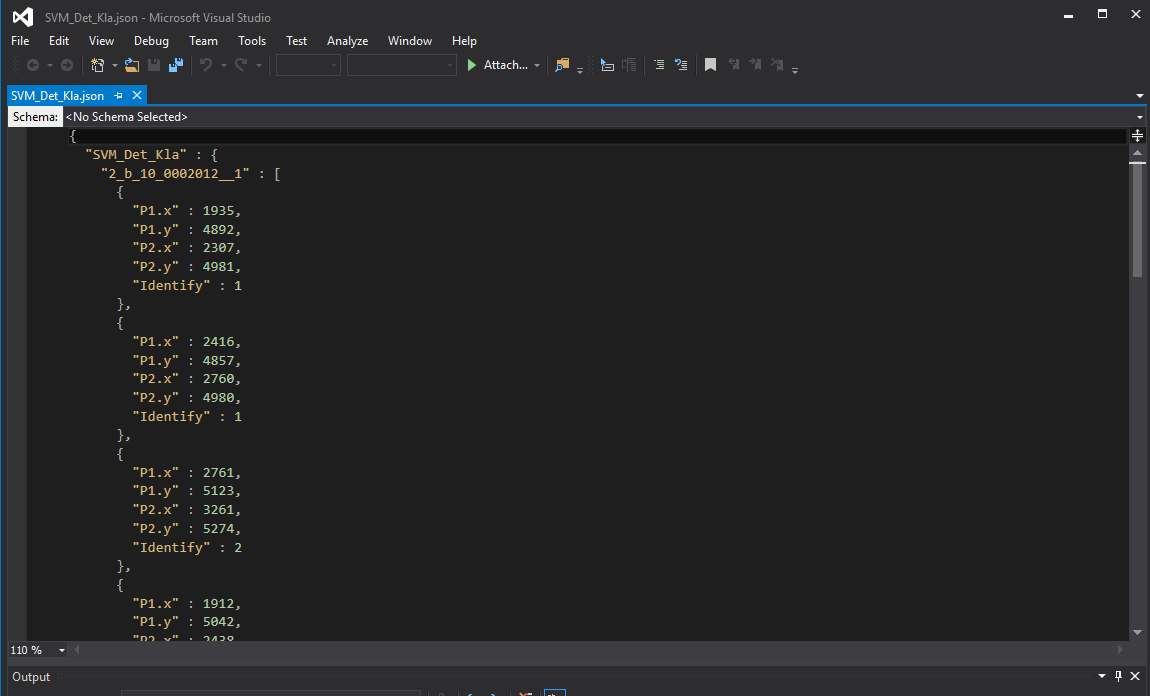
\includegraphics[width=0.5\textwidth]{Json.png}
	\caption{Beispiel für Json String}
	\label{fig:Bild 3.14}
\end{figure}
Danach werden alle ausgeschnitten Objekte wieder in OCR Server eingeworfen, noch mal feine text Mining zu schaffen, um das Ergebnis zu verbessern.

\chapter{Zusammenfassung}

\section{Erfahrungsgewinnen}
Diese Arbeitstätigkeit bietet für mich die Gelegenheit, in einen Beruf, eine Team 'hineinzuschnuppern'. Dabei habe ich wichtige Erfahrungen gesammelt und herausgefunden, in welchem Bereich ich gearbeitet habe. Gleichzeitig bietet sich für diese Arbeitstätigkeit die Chance, ich intensiv kennenzulernen. So kann wertvolle Kontakte für die Zukunft entstehen. Meine Erwartung an diese Arbeitstätigkeit war sehr deutlich, dass ich die während meines Studium in China erworbenen Programmierkenntnisse anwenden und speziell in C\# und .NET viel auszunutzen und weiter lernen und die Kenntnisse von Bildverarbeitung mehr kennenzulernen. 
Aufgrund fast drei Jahre Teiltätigkeiten in diesem Projekt an der Hochschule Hannover habe ich insgesamt ein enormer Erfahrungsgewinn. Dies bezieht sich vor allem auf die inhaltliche Auseinandersetzung mit den Themen Bildverarbeitung, Objekterkennung, Machine Learning und Daten Bank. Diese Tätigkeit erweiterte mein Wissen, wie z.B. viele Sache muss eindenken, wenn eine Gruppe zusammen arbeiten, VCS (Version Control System) wurde sehr nützlich. Bei den Besprechungen mit Fachkräften und Kollegen, die zur aktuellen und geplanten Arbeiten und bei Veranstaltungen stattfanden, wurde für mich insbesondere deutlich, wie die Prozesse nicht nur in unserem Team Hochschule Hannover sondern auch in allen Partnern an diesem Projekt laufen, z.B. monatlich Tele-Konferenz. Außerdem lernte ich, wie wichtig das Dokumentiren von vorgängigen und aktuellen Arbeiten, und eine gute Abteilung ist sehr wichtig, weil sonst werden die Mitarbeiter/Mitarbeiterin wurden immer Doppel-Arbeiten erledigen. Es wird sehr stark Arbeitsablauf beeinflussen. 


\section{Auswirkungen auf die eigene Berufsvorstellung}
Das Praktikum in einer Automobilelektronikeinrichtung war auch mit dem Ziel verbunden, für meine zukünftige Berufsvorstellung Erfahrungen zu sammeln. Durch mein absolviertes Praktikum von Oktober 2016 bis April 2017 in der BMW konnte ich erste Eindrücke vom Berufsfeld Erprobung Gesamtfahrzeug gewinnen. Dies motivierte mich so sehr, dass ich ein Praktikum in der Autoindustrie machen wollte. Dadurch sollte sich das Interesse für meinen späteren Berufswunsch konkretisieren lassen. Dies ist insbesondere für einen Studenten der Elektrotechnik wichtig, weil die Themenbereiche und Arbeitsplatzmöglichkeiten weit gefächert sind. Deswegen erscheint es mir wichtig zu wissen, in welchem Bereich der Erprobung Gesamtfahrzeug und mit welchen Inhalten ich in meinem Berufsleben arbeiten möchte.
Das Praktikum beim EG-CN-62 im Bereich Validation der E/E Komponente und Funktionentest hat dabei meine Erwartungen erfüllt und mich in meiner Berufsvorstellung bestätigt. Dies erscheint mir als reizvoll und sinnvoll. Die praktischere Erfahrung in diesem Bereich macht mich nicht nur im Bereich der Erprobung Gesamtfahrzeug sondern auch in fast allen Bereichen über E/E System für mein Berufsleben konkurrenzfähig, da ich mich auch mit anderen Abteilungen beschäftigt habe, die nur spezielle E/E Komponenten bearbeiten.


\section{Bewertung der eigenen Leistungen}
 Initiative, Leistungswillen, Fleiß und Arbeitsmoral waren ich während des gesamten Arbeitsraum immer bei mir. Die Akzeptanz meiner Persönlichkeit und meine berufliche Fähigkeit wurden von allen Kollegen, die in meinem Team und in anderen Abteilungen arbeiten, gefördert. Ich fühlte mich stets gefordert und habe deswegen auch meine Motivation bis zum Ende halten können. Bei der Durchführung des Softwareentwicklung und Compute Vision habe ich mich am Anfang des Arbeit manchmal unsicher gefühlt, weil die Schritte dafür sich teilweise als schwierig und eigenartig gestaltet haben. Dies konnte ich aber im Laufe meiner Arbeit entschärfen, indem ich über die Schritte und Methode nochmals mit meinem Team diskutiert habe und um Rat gefragt habe. Dadurch konnten weitere Schritte geklärt werden. Bei der Lösung dieses Problems möchte ich allen Kollegen danken, da sie ihre Erfahrungen mit mir ausgetauscht haben. Das erlaubte mir, ein Problem mit unterschiedlichen Lösungen zu behandeln. Trotz dieser kleineren Schwierigkeiten habe ich mich bei der Erfüllung meiner Aufgaben wohl gefühlt und mich von meiner Seite gut in das Team integriert. Mein Team erlaubte mir, für ein Fahrzeug, Mini Cooper Clubman (Siehe Abb. 17) vollständig die Verantwortung zu übernehmen. Jedes Mal, wenn ich auf ein Problem traf, boten Sie mir ausgezeichnete Lösungen an. Danke für das Vertrauen und großzügige Unterstützung von meinem Team. 

\section{Rückmeldung des Arbeitgebers}
Zum Ende meines Praktikums hat ein Abschlussgespräch mit meinem Betreuer und dem Team stattgefunden, in dem ich meine Erfahrungen reflektieren sollte und eine Bewertung meiner Arbeitsleistung erhalten habe. Hierbei ging es vordergründig um die Aufgabe der Validation der E/E Komponente laut der I-Stufe und die Funktionentests laut EHB. Dabei wurde besonders hervorgehoben, dass meine Arbeitsleistung im FIT Team sehr gut war. Von meinem Betreuer wurde des Weiteren geschätzt, dass ich eigene Ideen und Vorstellungen in meine Arbeit eingebracht habe und die mir gestellten Aufgaben eigenständig ausgeführt habe.

\section{Zusammenfassung der Tätigkeit}
Das Praktikum war auf der inhaltlichen Ebene für mich ein interessanter Bereich, da während meines Elektrotechnikstudiums eine sehr enge Auseinandersetzung mit den Themen Validation der E/E Komponente und Funktionentests stattgefunden hat.
Bei der Bearbeitung der Validation der E/E Komponente und den Funktionentests konnte ich an meine Erfahrungen aus dem Studium anknüpfen. Die Kenntnisse über Automobilelektronik habe ich nutzen können um meine Arbeitsaufgabe strukturiert und kompetent gestalten zu können. Die Theorie, die ich aus Fachliteratur und Vorlesungen gelernt habe, ist abstrakt und nicht einfach zu verstehen. Das Praktikum erlaubte mir, die E/E Komponenten in der Realität kennenzulernen. Nun kann ich die Theorie besser verstehen und die vorherigen Missverständnisse vermeiden. Die Fachliteratur lässt mich auf der theoretischen Ebene verstehen, wie die E/E Komponente funktioniert und mit welchen mechatronischen Elementen sie verbunden werden muss, um die Funktionen des Fahrzeugs zu realisieren. Nachdem die Fachkraft in meinen Team den Grundsatz der Automobilelektronik ausführlich erläutert hat, muss ich einmal reflektieren, welche Unterschiede zwischen der Theorie in der Literatur und dem aktuellen Wissensstand bestehen, denn die Lehrmeinungen der Literatur sind teilweise überholt.

\printbibliography
	                      	
\end{document}   